\documentclass[times, utf8, zavrsni, numeric]{fer}
\setlength{\parindent}{0em}
\tolerance=1
\emergencystretch=\maxdimen
\hyphenpenalty=10000
\hbadness=10000
\graphicspath{{../Slike/}}
\usepackage{hyperref}
\hypersetup{
	colorlinks=true,
	citecolor=black,
	linkcolor=black,
	urlcolor=cyan,
	pdflinkmargin=5pt
}

\begin{document}

% TODO: Navedite broj rada.
\thesisnumber{000}

\title{POVEZIVANJE VIRTUALNOG I STVARNOG OSVJETLJENJA KORIŠTENJEM UNREAL SUSTAVA}

\author{Bernard Bačani}

\maketitle

% Ispis stranice s napomenom o umetanju izvornika rada. Uklonite naredbu \izvornik ako želite izbaciti tu stranicu.
\izvornik

% Dodavanje zahvale ili prazne stranice. Ako ne želite dodati zahvalu, naredbu ostavite radi prazne stranice.
\zahvala{Zahvaljujem se Tiboru Jakovecu što je svaki dan išao sa mnom u menzu i svaki dan kasnio.}

\tableofcontents

\chapter{Uvod}

\chapter{Virtualna produkcija}
Filmska produkcija je izuzetno kompleksan proces koji je tipično linearan te se sastoji od razvoja, pretprodukcije, produkcije i postprodukcije (slika \ref{fig:slika 2-1}). Problem tradicionalne produkcije je izoliranost sudionika u pojedinoj fazi i neprilagodljivost promjenama na samom setu. Konačna verzija scene ne zna se do samog kraja produkcije, što uvelike otežava cijeli proces snimanja.\newline

\begin{figure}[htp]
	\centering
	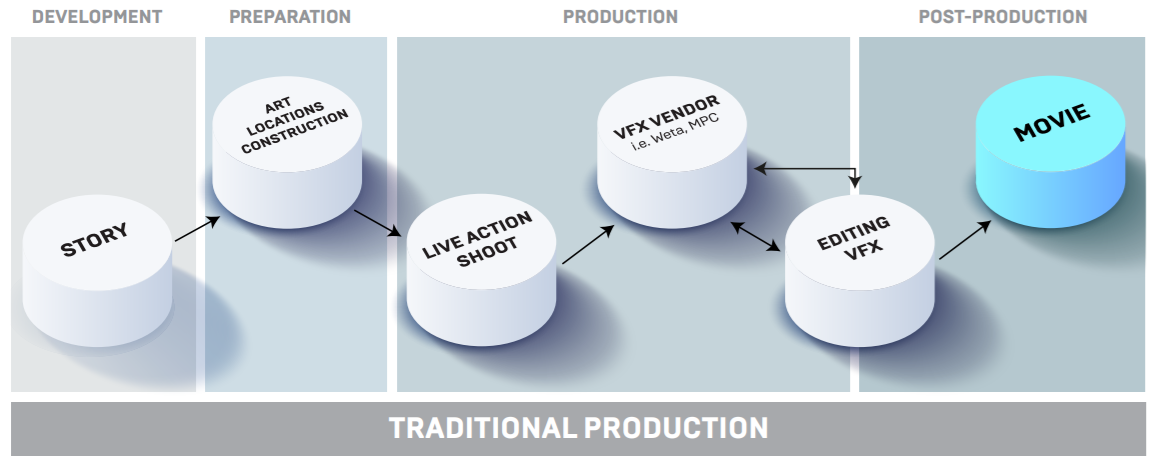
\includegraphics[width=\linewidth]{slika 2-1.png}
	\caption{Tradicionalna produkcija \cite{vpguide1}}
	\label{fig:slika 2-1}
\end{figure}

Virtualna produkcija je metoda slična agilnom razvoju, gdje se korištenjem pogonskog sklopa igara (engl. \emph{game engine}) prati kretnja kamere u stvarnom vremenu te se pozadinski sadržaj prikazuje na LED ekranu. Za razliku od tradicionalne, virtualna produkcija uvodi fleksibilnost u snimanje, omogućujući promjenu priče ili bilo kojeg dijela seta uz prisutnost cijelog tima, čime se štedi na vremenu i resursima (slika \ref{fig:slika 2-2}).

\pagebreak

\begin{figure}[htp]
	\centering
	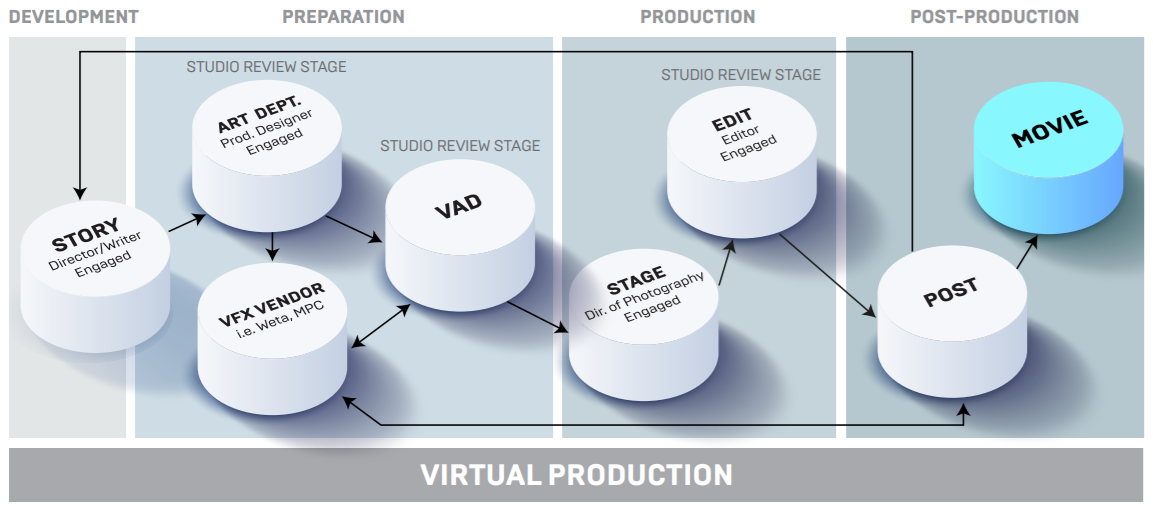
\includegraphics[width=\linewidth]{slika 2-2.png}
	\caption{Virtualna produkcija \cite{vpguide1}}
	\label{fig:slika 2-2}
\end{figure}

\section{Slučajevi upotrebe}
Vizualizacija je vjerojatno najčešći oblik upotrebe virtualne produkcije, a posebice predvizualizacija, koja u novoj paradigmi pruža prvi uvid u ideje i sredstva koja će se koristiti kroz produkciju \cite{vpguide2}. Poznata uporaba ove tehnike je u seriji \emph{The Mandalorian} (2019.-) gdje je virtualna produkcija bila korištena u snimanju više od pola cijele prve sezone (slika \ref{fig:slika 2-3}).\newline

Osim u filmovima i serijama može se koristiti u predvizualizaciji raznih javnih događaja poput koncerata. Primjerice, tvrtka Moment Factory je u 2021. godini objavila projekt \emph{DMX Previs}, digitalni svjetlosni šou (engl. \emph{light show}) napravljen koristeći DMX plugin u Unrealu (slika \ref{fig:slika 2-4}) koji je sličan primjeru iz stvarnog života te ga se može i upravljati upravljačkom konzolom za osvjetljenje.\newline

Također, virtualna produkcija koristi se za hvatanje pokreta (engl. \emph{motion capture}) - praćenja pokreta objekata ili glumaca za animaciju digitalnih modela i kod vizualnih efekata u kameri (engl. \emph{in-camera visual effects}, skraćeno in-camera VFX).

\begin{figure}[htp]
	\centering
	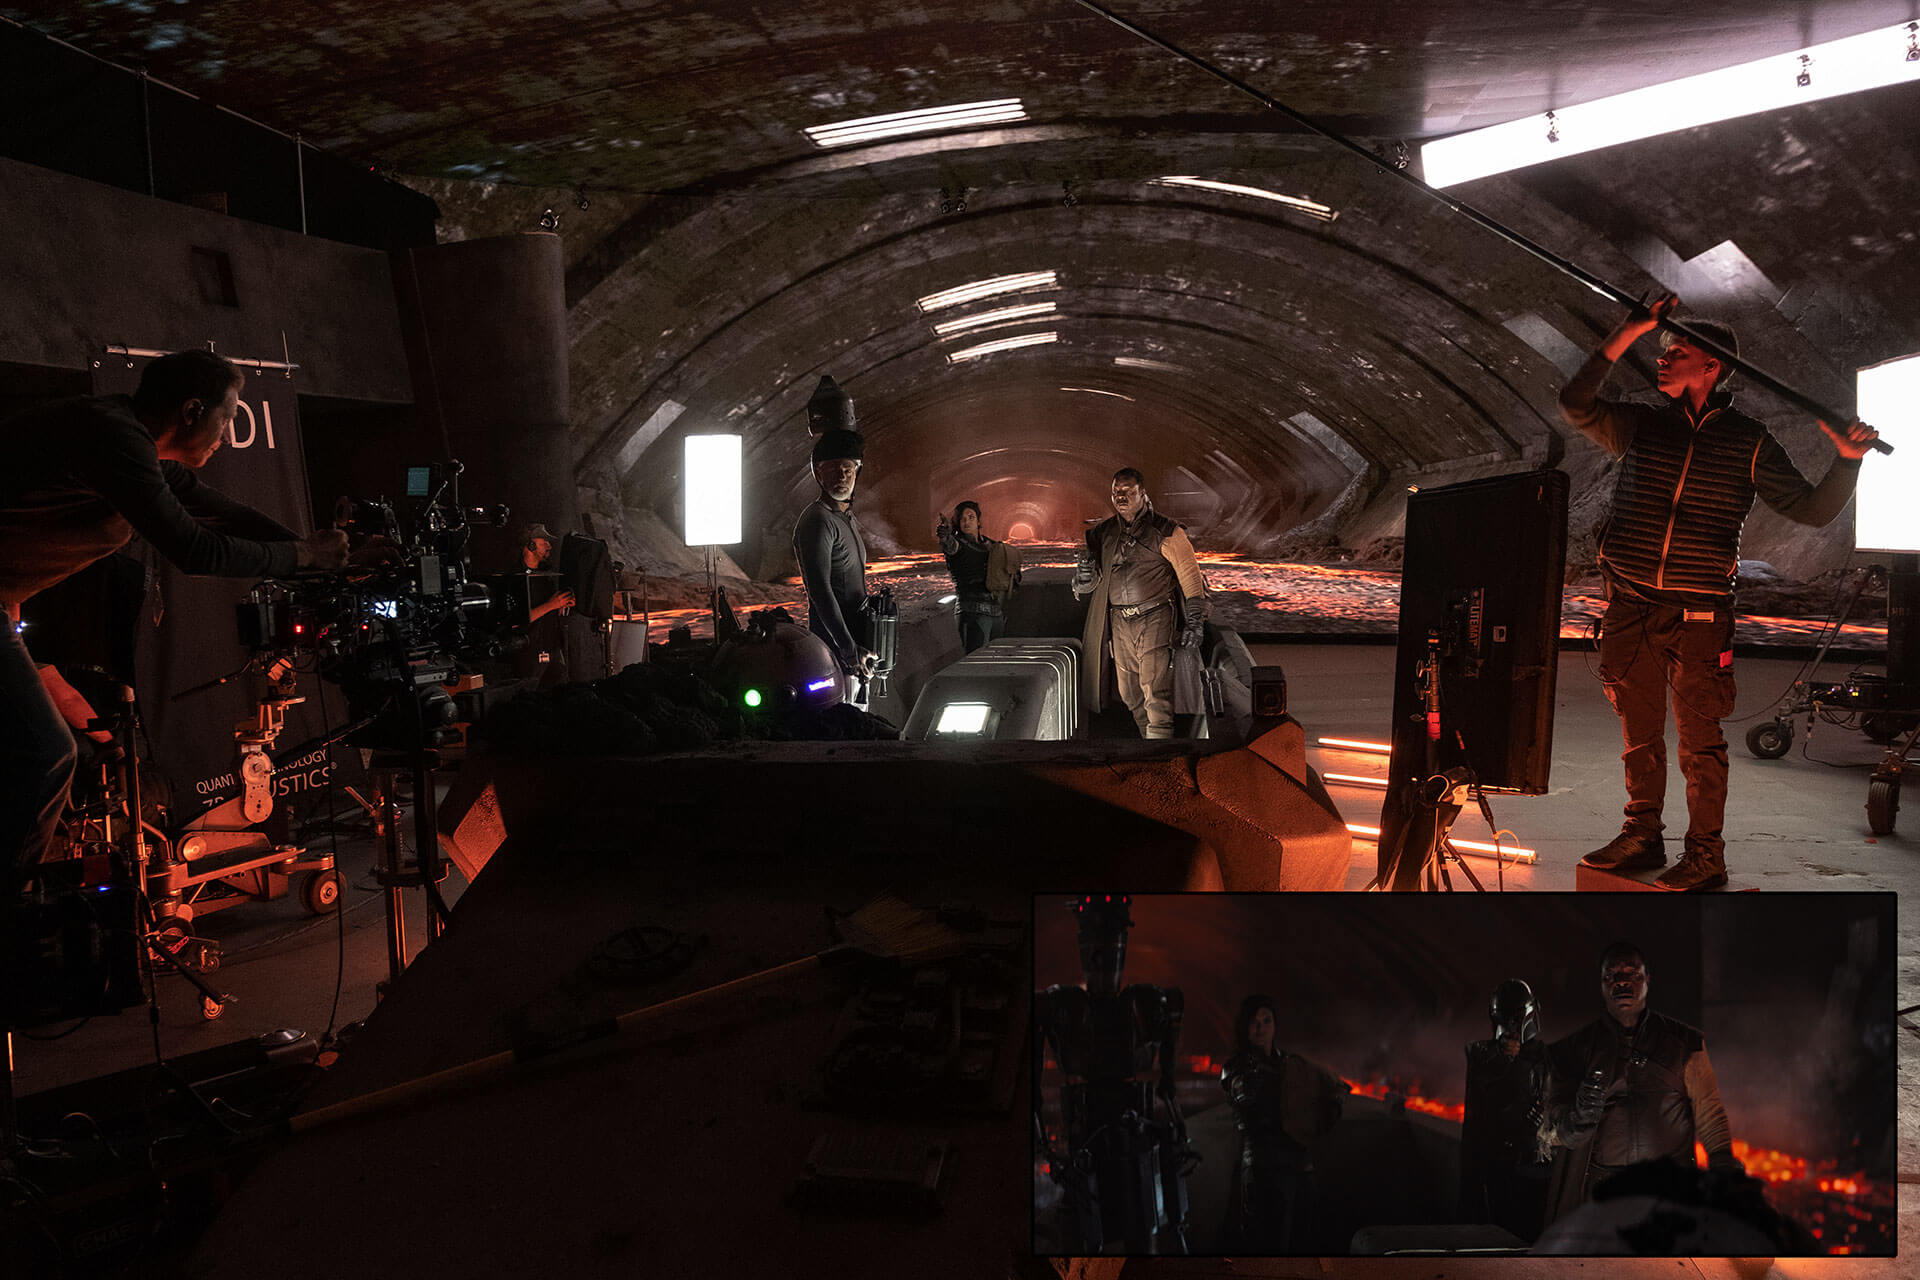
\includegraphics[width=\linewidth]{slika 2-3.png}
	\caption{Set u seriji \emph{The Mandalorian} \cite{mandalorian}}
	\label{fig:slika 2-3}
\end{figure}

\begin{figure}[htp]
	\centering
	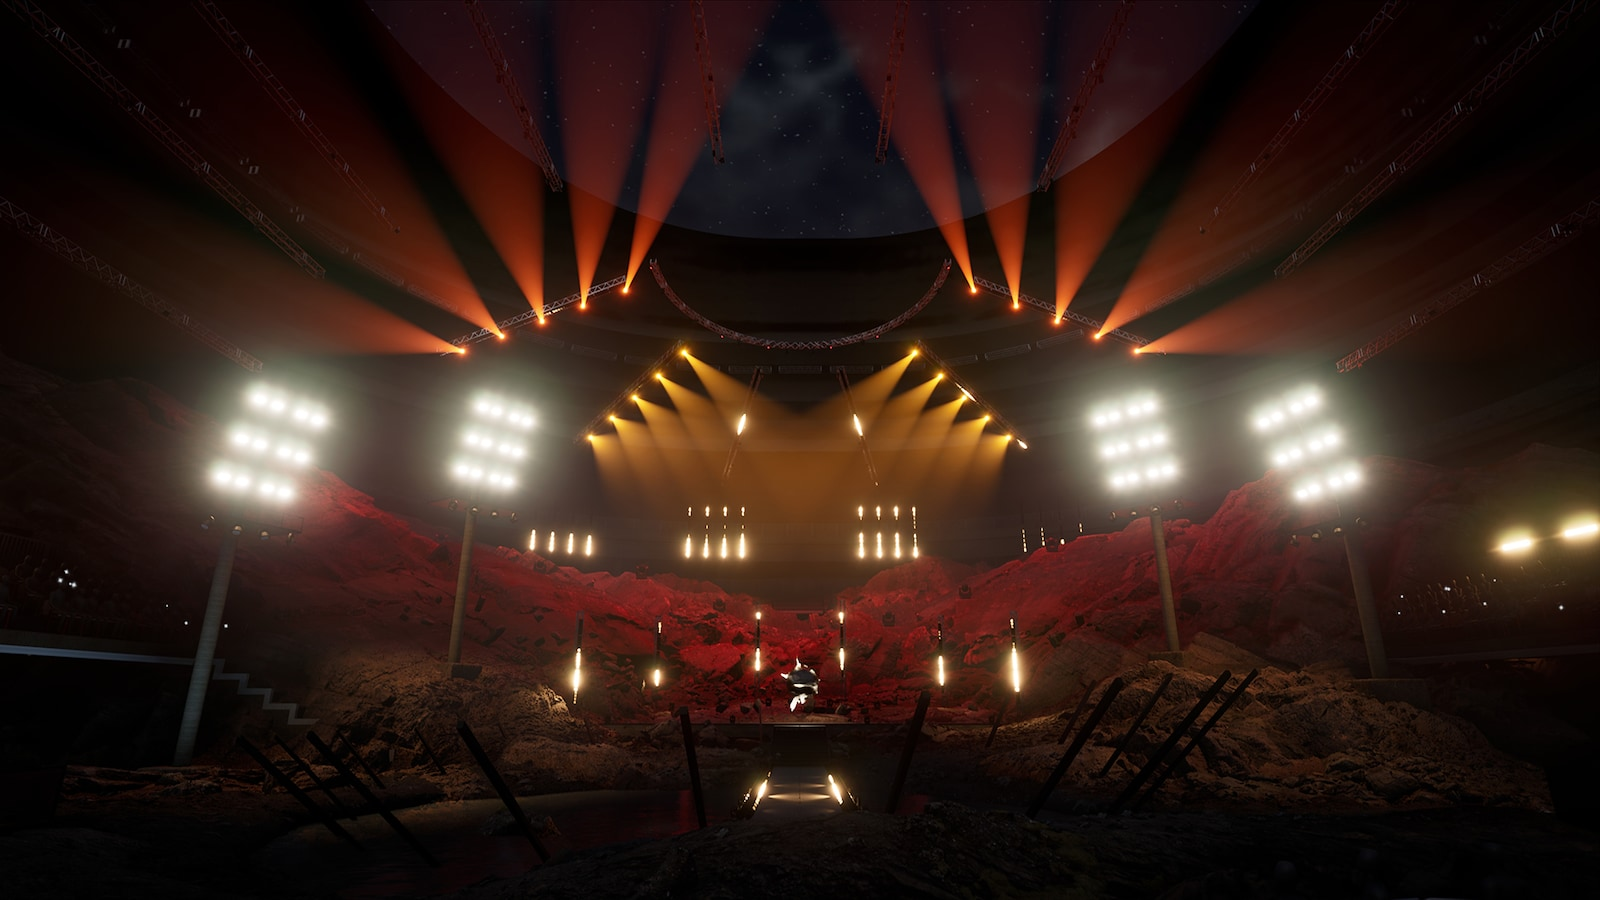
\includegraphics[width=\linewidth]{slika 2-4.png}
	\caption{Svjetlosni šou \emph{DMX Previs} \cite{dmx_previs}}
	\label{fig:slika 2-4}
\end{figure}

\pagebreak

\section{Opis prototipa}

\chapter{Upravljanje osvjetljenjem}
Za upravljanje osvjetljenjem u industriji se koristi konzola za upravljanje rasvjetom, elektronički uređaj koji komunicira sa svjetlima, prigušivačima i ostalim specijalnim efektima putem protokola upravljanja. Osim komuniciranja direktno, neke konzole mogu komunicirati s uređajima putem mreže pomoću mrežnih protokola.

\section{DMX}
Digital Multiplex (skraćeno DMX) je standardni digitalni komunikacijski protokol koji se uobičajeno koristi za upravljanje svjetlima i svjetlosnim efektima dajući im naredbe poput promjene boje, pozicije i intenziteta. Izvorno namijenjen kao standardna metoda za kontrolu prigušivača svjetlosti, brzo je proširio svoju namjenu na kontrolu ostalih uređaja, poput vatrometa, lasera, mikrokontrolera, inteligentna svjetla, uređaja za maglu itd.

DMX možemo gledati kao paket digitalnih informacija koji se šalju s izvora na odredište pri čemu svaki paket sadrži polje od 512 bajtova čije su vrijednosti između 0 i 255 (slika \ref{fig:slika 3-1}).

\begin{figure}[htp]
	\centering
	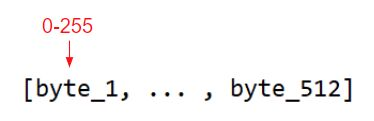
\includegraphics[width=\linewidth]{slika 3-1.png}
	\caption{DMX paket \cite{dmx_overview}}
	\label{fig:slika 3-1}
\end{figure}

\subsection{Kontroleri}
DMX kontroleri (engl. \emph{controllers}) djeluju kao izvor DMX paketa te šalju podatke do jednog ili više povezanih uređaja. Postoje dva oblika DMX kontrolera, USB/mrežno sučelje koje pretvara USB signale ili IP pakete u DMX te standardna DMX konzola koja omogućuje ručno aktiviranje slanja DMX paketa. Konzole također mogu imati podršku za komunikaciju preko mreže.

\subsection{Rasvjetni uređaji}
DMX rasvjetni uređaji (engl. \emph{fixtures}) su uređaji koji primaju DMX pakete te na temelju primljenih podataka obavljaju određenu naredbu. Naredbe mogu biti razne, obično uključivanje/isključivanje, pojačavanje/smanjivanje intenziteta, promjena boje te rotacija za neki kut.

Svaki rasvjetni uređaj ima niz atributa koji su unaprijed definirani na hardverskoj razini te su organizirani u grupe koje zovemo odama (engl. \emph{odes}). Često uređaji imaju više načina rada (engl. \emph{mode}) kako bi korisnici mogli odabrati samo one funkcije koje im zaista trebaju te time pojednostavili upravljanje. Npr. ako neki uređaj ima ugrađenih 8 funkcija, a način rada mu se postavi na 4 kanalni, tada će samo prve 4 funkcije biti dostupne.

Svemir (engl. \emph{universe}) u DMX-u predstavlja niz spojenih rasvjetnih uređaja koje čitaju iste podatke (pakete). Svaki svemir sadrži 512 adresa te se na jedan svemir može spojiti najviše 512 rasvjetnih uređaja (uz pretpostavku da su svi uređaji 1 kanalni). Dakle, rasvjetni uređaj će zauzimati onoliko adresa u svemiru koliko atributa ima u trenutnom načinu rada (4 kanalni način rada = 4 adrese).

\subsection{Komunikacija signala}
Svaki kontroler je zadužen za jedan ili više svemira te u svakom svemiru se nalazi nekoliko rasvjetnih uređaja. Kada kontroler šalje DMX paket, locira svemir kojemu ga treba poslati te šalje isti paket svakom rasvjetnom uređaju u tom svemiru. Paket se šalje slijedno, prvi uređaj pročita podatke u paketu te šalje paket dalje sljedećem. Kako bi uređaj pravilno primio podatke koji se odnose na njega, treba slušati odgovarajuće podatke u paketu, zbog čega je uvedeno adresiranje.

Adresiranje (engl. \emph{fixture patching}) svakom rasvjetnom uređaju dodjeljuje specifičnu početnu adresu u svemiru, čime rasvjetni uređaj tada zauzima raspon adresa od početne adrese do početne adrese plus koliko je atributa u trenutnom načinu rada (slika \ref{fig:slika 3-2}).

\pagebreak

\begin{figure}[htp]
	\centering
	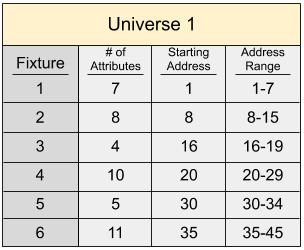
\includegraphics[width=\linewidth]{slika 3-2.png}
	\caption{Adresiranje \cite{dmx_overview}}
	\label{fig:slika 3-2}
\end{figure}

Prema primjeru na slici, kada se pošalje DMX paket, rasvjetni uređaj 4 će od 512 adresa u paketu slušati samo one na adresama 20-29, a ostale će zanemariti.

Većinu vremena atributu će biti dovoljan opseg unosa od jednog bajta (0-255), ali ako želimo veću kontrolu te jedan bajt nije dovoljan, atribut može zauzeti više adresa u svemiru. Primjerice, atribut koji zauzima dvije adrese može poprimiti vrijednosti u rasponu 0-65,536. Ostali primjeri:

\begin{enumerate}
	\item 8-bitni atribut - Min: 0, Max: 255 - zauzima 1 adresu
	\item 16-bitni atribut - Min: 0, Max: 65,536 - zauzima 2 adrese
	\item 24-bitni atribut - Min: 0, Max: 16,777,215  - zauzima 3 adrese
	\item 32-bitni atribut - Min: 0, Max: 4,294,967,296  - zauzima 4 adrese
\end{enumerate}

\section{Mrežni protokoli}
Porastom kompleksnosti i broja uređaja korištenih u predstavama pojavila se potreba za lakšim i bržim adresiranjem i upravljanjem rasvjetnim uređajima. Napretkom komunikacijskih tehnologija razvijeni su ethernet protokoli koji omogućuju prijenos više DMX svemira putem Cat5 kabla. Unreal Engine podržava dva ethernet protokola, Art-Net i sACN.
\subsection{Art-Net}
Art-Net je ethernet protokol temeljen na paketu protokola TCP/IP te se koristi za prijenos velikog broja DMX paketa putem UDP protokola. Najnovija revizija je Art-Net 4 i podržava prijenos 32,768 svemira (teoretski, stvarni broj ovisi o fizičkom sloju mreže i metodi prijenosa) i preko 1000 DMX priključaka (engl. \emph{ports}), gdje je adresa priključka svakog svemira kodirana kao 15-bitni broj (slika \ref{fig:slika 3-3}).

\begin{figure}[htp]
	\centering
	\includegraphics[width=\linewidth]{slika 3-3.png}
	\caption{Adresa priključka svakog DMX svemira \cite{art-net}}
	\label{fig:slika 3-3}
\end{figure}

Podmreža (engl. \emph{Sub-Net}) je grupa od 16 uzastopnih svemira, a mreža (engl. \emph{Net}) je grupa od 16 uzastopnih podmreža ili 256 uzastopnih svemira.

Kod prvog spajanja mreže, kontroleri ne znaju broj uređaja u mreži ni njihove IP adrese te se za njihovo otkrivanje koristi broadcast - kontroler pošalje ArtPoll paket na IP adresu 2.255.255.255 na UDP priključku 0x1936. ArtPoll paket šalje samo kontroler, a odgovor ArtPollReply šalju i kontroleri i uređaji. Maksimalno vrijeme čekanja između slanja ArtPoll paketa i primanja ArtPollReply paketa je 3 sekunde. Kontroler koji je poslao ArtPoll paket bi također trebao odgovoriti na svoju poruku sa ArtPollReply, čime se osigurava da bilo koji drugi kontroleri koji slušaju na mreži detektiraju sve uređaje bez potrebe da svaki spojeni kontroler šalje ArtPoll paket. Svi kontroleri moraju poslati ArtPoll svakih 2.5 do 3 sekunde, čime se lako otkriva prekid veze. 

Za prijenos DMX podataka koristi se unicast ili broadcast te se šalje ArtDmx podatkovni paket (slika \ref{fig:slika 3-4}).

\begin{figure}[htp]
	\centering
	\includegraphics[width=\linewidth]{slika 3-4.png}
	\caption{Prijenos DMX paketa \cite{streaming_packets}}
	\label{fig:slika 3-4}
\end{figure}

Iako se za slanje ArtDmx može koristiti broadcast, u velikom sustavu dolazi do ogromnog opterećenja obrade podataka te se koristi unicast. Kako bi se mogao koristiti unicast, kontroleri trebaju znati  koji uređaji slušaju na određenom priključniku, što se ostvaruje preplatom (engl. \emph{subscription}) \cite{subscription}. Pretplata se odvija na sljedeći način:

\begin{enumerate}
	\item Kontroler broadcast šalje ArtPoll svakih 2.5 do 3 sekunde.
	\item Kontroler analizira sve ArtPollReply pakete i sastavlja popis do 8 mogućih priključnih adresa i pridružene IP adrese za svaki uređaj koji odgovori (pretplatnici).
	\item Kontroler koristi ovaj popis za izračunavanje IP adrese koju bi trebao koristiti za unicast slanje ArtDmx paketa.
\end{enumerate}

ArtSync paket koristi se za sinkronizaciju slanja ArtDmx paketa. Sinkronizacija se odvija tako da kontroler unicast šalje više ArtDmx svemira, a zatim broadcast pošalje jedan ArtSync paket koji javlja da je zadnji ArtDmx paket stigao.

\pagebreak

\subsection{sACN}
Arhitektura strujanja za upravljačke mreže (engl. \emph{Streaming Architecture for Control Networks}, skraćeno sACN) je standardni protokol razvijen za efikasni prijenos DMX svemira preko mreže. Konceptualno je veoma usporediv s Art-Netom te se sastoji od podatkovni paket (E1.31 Data Packet) za prijenos DMX podataka, paket otkrivanja (E1.31 Universe Discovery Packet) za praćenje prometa i sinkronizacijski paket (E1.31 Synchronization Packet). Za razliku od Art-Neta, podržava prijenos do 63,999 svemira i multicast, čime se mogu prenositi podaci bez prethodnog znanja topologije mreže \cite{sACN}.

\section{GDTF}
General Device Type Format (skraćeno GDTF) protokol je otvoreni standard razvijen kako bi se olakšala primjena novih rasvjetnih uređaja (slika \ref{fig:slika 3-5}). GDTF datoteka je otvorenog formata te se sastoji od XML datoteke koja sadrži informacije o pojedinom uređaju poput geometrije, atributa, načina rada i pretpostavljenih vrijednosti \cite{dmx_gdtf}. Baza podataka svih dostupnih GDTF datoteka je besplatna \cite{GDTF}.\\

\begin{figure}[htp]
	\centering
	\includegraphics[width=\linewidth]{slika 3-5.png}
	\caption{GDTF \cite{dmx_gdtf}}
	\label{fig:slika 3-5}
\end{figure}

\chapter{Model rješenja}
Upravljačka konzola za osvjetljenje je uređaj kojim se upravlja svjetlosnim i drugim uređajima putem upravljačkog protokola. Zbog povećane količine uređaja na pozornici, osim komuniciranja direktno ili preko USB-a, neke konzole također mogu komunicirati putem mreže kako bi se olakšala kontrola nad složenim sustavima. Za ovaj rad korišten je simulator konzole koji šalje podatke preko ethernet protokola.\newline

Svjetlosni efekti korišteni u simulaciji su nalik na one u javnima događajima, poput koncerata gdje se koriste primjerice reflektori, laseri, dimni efekti i drugo.
Zatim, simulacija se integrira s postojećim sustavom za detekciju položaja kamere u kojem se pomoću stvarne kamere upravlja virtualnom kamerom u stvarnom vremenu.

\section{Simulacija osvjetljenja}
Simulacija je zamišljena kao predvizualizacija mini pozornice u kazalištu. Pozornica sadrži nekoliko reflektora, statičnih svjetala i lasera. Svjetlosnim uređajima se upravlja simulatorom konzole te se svjetla pale i gase, mijenja im se pozicija, pojačava ili smanjuje intenzitet i slično. Promatra se unaprijed programiran skup naredbi, a zatim slanje naredbi u stvarnom vremenu i njihovo kašnjenje. Simulacija je uspješna ako je dobiven rezultat sličan korištenju prave konzole te je utjecaj kašnjenja minimalan.

\pagebreak

\section{Integracija s prototipom}
Povezivanje s prototipom ostvaruje se korištenjem stvarne kamere, sustava za virtualnu stvarnost i LED zaslona. Kako se simulacija izvodi, kretanjem stvarne kamere mapiraju se pokreti u virtualnu kameru te se time krećemo po pozornici. Ispred LED zaslona stavljaju se objekti u stvarnom životu te se snima smješten objekt u virtualnoj sceni. Integracija je uspješna ako dobijemo dojam da se objekt stvarno nalazi na pozornici, a simulirana svjetlost nalikuje stvarnoj svjetlosti.

\chapter{Korištene tehnologije}

\chapter{Izrada simulacije osvjetljenja}

\chapter{Integracija s prototipom}

\chapter{Rezultati}

\chapter{Zaključak}

\raggedright
\bibliography{literatura}
\bibliographystyle{fer}

\begin{sazetak}
Sažetak na hrvatskom jeziku.

\kljucnerijeci{Ključne riječi, odvojene zarezima.}
\end{sazetak}

\engtitle{CONNECTING VIRTUAL AND REAL LIGHTING USING THE UNREAL SYSTEM}
\begin{abstract}
Abstract.

\keywords{Keywords.}
\end{abstract}

\end{document}
